\section{Model assessment and selection}
\textit{Take a look also at this: https://machinelearningmastery.com/probabilistic-model-selection-measures/}
\begin{definition}{\textbf{Training error}}: it is the average loss over the training samples:
\begin{equation}
\bar{err} = \frac{1}{N}\sum_{i=1}^N L(y_i, \hat{f}(x_i))
\end{equation}

For categorical variables it is:
\begin{equation}
\bar{err}  = -\frac{2}{N} \sum_{i=1}^N \log\hat{p}_k(x_i)
\end{equation}
The "$-2$" in the definition makes the log-likelihood loss for the Gaussian distribution match squared-error loss.
\label{trainErr}
\end{definition}

\begin{definition}{\textbf{Test error:}} with  the term \textit{test error} or \textit{generalization error} we indicate the prediction error over an independent test sample different from the one used for the training and it is indicated as 
\begin{equation}
Err_\tau \left[L(Y,\hat{f}(X)|\tau\right]
\end{equation}
where $\tau$ indicates the training set and $X$ and $Y$ are drawn randomly from their joint distribution.
\end{definition}

\begin{definition}{\textbf{Expected prediction error}}: or \textbf{expected test error} is the expectation of the test.
\begin{equation}
Err = \E\left[ L(Y,\hat{f}(X))\right] =  \E\left[Err_\tau\right]
\end{equation}
\end{definition}

\autoref{testErr} shows the prediction errors of the same type of model trained with different training sets in light red and their expectation (average) in dark red.

\begin{figure}
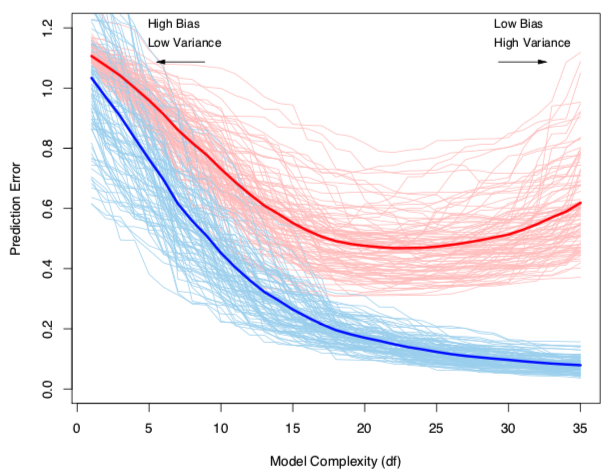
\includegraphics[scale=0.6]{img/testErr}
\caption{Behaviour of test sample and training sample error as the model complexity is varied. The light blue curves show the training error $\bar{err}$, while the light red curves show the conditional test error $Err_\tau$ for $100$ training sets of size $50$ each, as the model complexity is increased. The solid curves show the expected test error $Err$ and the expected training error $E[\bar{err}]$.}
\label{testErr}
\end{figure}
To judge the prediction capability of a model we need to estimate $Err_\tau$. As the model becomes more and more complex, it uses the training data more and is able to adapt to more complicated underlying structures. Hence there is a decrease in bias but an increase in variance. There is some intermediate model complexity that gives minimum expected test error. The training error is not reliable because it always decreases with the model complexity and with too much complexity it looses the capability to generalize.

The same holds for categorical variables (introduced in \autoref{trainErr}). Typical loss functions are:
\begin{equation}
\begin{aligned}
&L(G, \hat{G}) = I(G\ne\hat{G}(X)) \quad\quad \textit{0-1 loss},\\
&L(G, \hat{p}(X)) = -2\sum_{k=1}^K I(G=k)\log\hat{p}_k(X) \quad\quad \textit{-2 $\times$ log-likelihood},\\
\end{aligned}
\end{equation}
where the quantity $-2 \times \log-likelihood$ is generally referred as deviance. The "$-2$", as already said, in the definition makes the log-likelihood loss for the Gaussian distribution match squared-error loss.
A number of methods for estimating the expected test error for a model exists. Typically our model will have a tuning parameter or parameters $\alpha$ and so we can write our predictions as$ \hat{f}(x)_\alpha$
The tuning parameter varies the complexity of our model, and we wish to find the value of $\alpha$ that minimizes error, that is, produces the minimum of the average test error curve. There are two goals that one might want to achieve:
\begin{definition}{\textbf{model selection}}: estimating the performance of different models in order to choose the best one.
\end{definition}
\begin{definition}{\textbf{model assessment}}: having chosen a final model, estimate its prediction error on new data.
\end{definition}


If we are in a data-rich situation, the best approach for both problems is to randomly divide the dataset into three parts: a training set, a validation set, and a test set. The training set is used to fit the models; the validation set is used to estimate prediction error for model selection; the test set is used for assessment of the generalization error of the final chosen model. Ideally, the test set should be kept in a "vault", and be brought out only at the end of the data analysis. It is difficult to give a general rule on how to choose the number of observations in each of the three parts, as this depends on the signal-to-noise ratio in the data and the training sample size. A typical split might be 50\% for training, and 25\% each for validation and testing.

The following methods allows to work in a situation with insufficient data. The methods can be distinguished in analytical (AIC, BIC, MDL, SRM) or by efficiently sample re-use (cross-validation and boot-strap). 
Typically the more complex we make the model $f$, the lower the (squared) bias but the higher the variance.
\subsection{Optimism of the training error rate}
Given a training set $\tau$ the generalization error of a model is:
\begin{equation}
Err_\tau = \E_{X^0, Y^0}\left[ L(Y^0, \hat{f}(X^0))|tau\right]
\end{equation}
where the point $(X^0, Y^0)$ is a new test data point. Averaging over training sets $\tau$ (i.e., averaging over the same type of models $\hat{f}$ but trained with different trainsets belonging to the same distribution):
\begin{equation}
Err = \E_\tau \E_{X^0, Y^0}\left[ L(Y^0, \hat{f}(X^0))|tau\right]
\end{equation}
The training error $\bar{err} = \frac{1}{N}\sum_{i=1}^N L(y_i, \hat{f}(x_i))$  will be less than the true error, because the same data is being used to fit the method and assess its error. A fitting method typically adapts to the training data, and hence the apparent or training error $\bar{err}$ will be an overly optimistic estimate of the generalization error $Err_\tau$, which can be thought as \textit{extra-sample error}. 

The nature of the optimism in the training error can be explained considering the \textit{in-sample error}:
\begin{equation}
Err_{in} = \frac{1}{N} \sum_{i=1}^N E_{Y^0}\left[ L(Y_i^0, \hat{f}(x_i))|\tau\right]
\end{equation}
To explain it better consider the same input points $x_i, \quad i=1,\cdots, N$. In the training set for these points we got a given set of values, while on new data we get a slightly different values $Y^0$ due to the random process involved (for example the noise considering the additive model). The model $\hat{f}$ have been trained using the training set, so for its prediction for those points will be close to the values seen in the training set (influenced by randomness) and it cannot foresee the non-deterministic part in the new samples. We define the optimism as the difference between the real $Err_{in}$ and the training error:
\begin{equation}
op \equiv Err_in - \bar{err}
\end{equation} 
and this is typically positive since the second term is generally biased downward. Averaging the optimism:
\begin{equation}
\omega = \E_y(op)
\end{equation}
where the notation $\E_y$ has been used instead of $\E_\tau$ because the predictors (the inputs) are fixed, while the outputs vary.

For squared error, 0-1 loss functions and other loss functions one can show:
\begin{equation}
\omega = \frac{2}{N} \sum_{i=1}^N Cov(\hat{y_i}, y_i)
\end{equation}
Thus the amount by which err underestimates the true error depends on how strongly $y_i$ affects its own prediction. The harder we fit the data, the greater the covariance will be, thereby increasing the optimism. We have the relationship:
\begin{equation}
\E_y (Err_{in}) = \E_y(\bar{err}) +\frac{2}{N} \sum_{i=1}^N Cov(\hat{y_i}, y_i)
\end{equation}
This expression simplifies if $\hat{y}_i$ is obtained by a linear fit with d inputs or basis functions. For example for the additive model $Y=f(X) + \epsilon$:
\begin{equation}
 \sum_{i=1}^N Cov(\hat{y_i}, y_i) = d\sigma_\epsilon^2
\end{equation}
and so
\begin{equation}
\E_y (Err_{in}) = \E_y(\bar{err}) +\frac{2d}{N} \sigma_\epsilon^2
\label{paramSel}
\end{equation}
We can use these expressions to select the effective number of parameters. The optimism increases with the number $d$ of inputs or basis functions we use, but decreases as the training sample size increases

An obvious way to estimate prediction error is to estimate the optimism and then add it to the training error. The methods such as Cp, AIC, BIC and others work in this way, for a special class of estimates that are linear in their parameters.
In contrast, cross-validation and bootstrap methods are direct estimates of the extra-sample error. These general tools can be used with any loss function, and with nonlinear, adaptive fitting techniques.
In-sample error is not usually of direct interest since future values of the features are not likely to coincide with their training set values. But for comparison between models, in-sample error is convenient and often leads to effective model selection. The reason is that the relative (rather than absolute) size of the error is what matters.

\subsection{$C_p$ metric}
One can estimate the in-sample error as
\begin{equation}
\hat{Err} = \bar{err}+\hat{\omega}
\end{equation}
where $\hat{\omega}$ is an estimate of the average optimism. Using \autoref{paramSel}:
\begin{equation}
C_p = \bar{err} +\frac{2d}{N} \hat{\sigma}_\epsilon^2
\end{equation}
where $\hat{\sigma}_\epsilon^2$ is an estimate of the noise variance.

The model with lowest $C_p$ should be selected.

\subsection{Akaike Information Criterion}
Suppose we have models $\CMcal{M}_1, \cdots, \CMcal{M}_k$ where each model is a set of densities:
\begin{equation}
\CMcal{M}_j = \left\lbrace p(y;\theta_j):\theta_j \in \Theta_j\right\rbrace.
\end{equation}
and we have data $Y_1,\cdots, Y_n$ drawn from an unknown density $f$ that we do not know if it is in any of the models. Let $\hat{\theta}_j$ be the Maximum Likelihood estimation from the model $j$. Using this we can estimate $f$ with $\hat{p}_j(y) = p(y, \hat{\theta}_j)$. The quality of $\hat{p}_j(y)$ (i.e., its distance form $f$) can be measured by the \textbf{Kullback-Leibler distance}:
\begin{equation}
\begin{aligned}
K(p, \hat{p}_j) &= \int p(y) \log \frac{p(y)}{\hat{p}_j(y)} dy = \\
&=\int p(y) \log p(y) dy  - \int p(y) \log \hat{p}_j(y) dy 
\end{aligned}
\end{equation}
We want to minimize this distance. The first term is constant while we can act on $ \hat{p}_j(y)$. Since it is a probability (i.e.  $\hat{p}_j(y)$ is at most one, minimizing the distance is equivalent to maximizing the second term:
\begin{equation}
K_j = \int p(y) \log \hat{p}_j(y) dy 
\end{equation}
Intuitively one estimate of $K_j$ might be:
\begin{equation}
\bar{K}_j = \frac{1}{N} \sum_{i=1}^N \log p_j(Y_i,\hat{\theta}_j)  = \frac{\ell_j(\hat{\theta_j})}{N} 
\end{equation}
i.e., assuming a uniform distribution. This estimation is very biased because data are being used twice: once for the MLE and the second one to calculate the integral. So we have $\bar{K}_j \ne K_j$. We want to find such difference.

Let us drop the index $j$ (i.e., we are considering just one model and not a set) and just use $K$ and $\bar{K}$. Let $\theta_0$ be the parameters that minimize $K(f,p(\cdot, \theta))$. So $p(y, \theta_0)$ is the closest density in the model to the true density. Let $\ell(y,\theta)=\log p (y, \theta)$ and let us define the \textbf{score} as:
\begin{equation}
s(y,\theta) = \frac{\partial \log p (y, \theta)}{\partial \theta}
\end{equation}
and let $H(y, \theta)$ be the matrix of second derivatives.
Let
\begin{equation}
Z_N = \sqrt{N}\br{\hat{\theta} - \theta_0}
\end{equation}
and recall (?) that :
\begin{equation}
Z_N \rightarrow \CMcal{N}(0, J^{-1}VJ^{-1})
\end{equation}
where 
\begin{equation}
\begin{aligned}
&J = -\E\left[ H(Y,\theta_0\right]\\
& V = Var(s(Y,\theta_0))
\end{aligned}
\end{equation}
Let 
\begin{equation}
S_N = \frac{1}{N}\sum_{i=1}^N s(Y_i, \theta_0)
\end{equation}
By the \textbf{Central Limit Theorem}, and recalling that $\theta_0$ is the value that minimizes $K$ (if it is a convex function then for this value the score is $0$ i.e., $0$ mean):
\begin{equation}
\sqrt{N}S_N \rightarrow \CMcal{N}(0, V)
\end{equation}
since 
\begin{equation}
\begin{aligned}
\Var\left[ \sqrt{N} S_n\right] &= \E\left[ \br{\sqrt{N} S_n - \cancel{\mu_{S_n}}}^2\right]= \\
&= N \E\left[ \br{\frac{1}{N}\sum_{i=1}^N s(Y_i, \theta_0)}^2\right] = \frac{1}{N} \E\left[ \br{\sum_{i=1}^N s(Y_i, \theta_0)}^2\right] =\\
&= \frac{1}{N}  \br{\sum_{i=1}^N \E\left[s(Y_i, \theta_0)\right]^2} =\frac{1}{N} NV=V
\end{aligned}
\end{equation}
Now $J$ is a scalar, considering the distribution $JZ_N$ where $Z_N \rightarrow\CMcal{N}(0, J^{-1}VJ^{-1})$, the result is still a distribution with $0$. For the variance let us use the property:
\begin{equation}
\begin{aligned}
&\Var\left[ JZ_N\right] = J(J^{-1}VJ^{-1})J^T = V\\
&\Rightarrow JZ_N \sim \CMcal{N}(0,V)
\end{aligned}
\label{varMul}
\end{equation}

By using \textbf{Taylor series expansion}:
\begin{equation}
K \approx \int p(y) \br{\log p(y, \theta_0) + \cancel{\br{\hat{\theta} - \theta_0}^Ts(y,\theta_0)}+\frac{1}{2}\br{\hat{\theta} - \theta_0}^TH(y,\theta_0)\br{\hat{\theta} - \theta_0}} dy
\end{equation}
The second term $\br{\hat{\theta} - \theta_0}^Ts(y,\theta_0)$ is $0$ because the score has $0$ mean. Defining 
\begin{equation}
K_0  = \int  p(y) \log p(y, \theta_0)dy
\end{equation}
we have:
\begin{equation}
\begin{aligned}
K &\approx K_0 + \frac{1}{\sqrt{N}}Z_N^T \int H(y,\theta_0) p(y) dy \frac{1}{\sqrt{N}}Z_N  = \\
& =K_0 + \frac{1}{\sqrt{N}}Z_N^T \int H(y,\theta_0) p(y) dy \frac{1}{\sqrt{N}}Z_N = k_0 -\frac{1}{2N} Z_N^TJZ_N
\end{aligned}
\end{equation}
Now applying the \textbf{Taylor series expansion} to $hat{K}$:
\begin{equation}
\bar{K}  \approx \frac{1}{N} \sum_{i=1}^N \br{\ell(Y_i,\theta_0) + \br{\hat{\theta} - \theta_0}^Ts(Y_i,\theta_0)} + \frac{1}{2}\br{\hat{\theta} - \theta_0}^TH(Y_i,\theta_0)\br{\hat{\theta} - \theta_0}
\end{equation}
Defining 
\begin{equation}
\begin{aligned}
&A_N = \frac{1}{N} \sum_{i=1}^N \ell(Y_i, \theta_0) - K_0 = \frac{1}{N} \sum_{i=1}^N \br{\ell(Y_i, \theta_0) - K_0}\\
&J_N = -\frac{1}{N} \sum_{i=1}^NH(Y_i,\theta_0) - \xrightarrow{P} J
\end{aligned}
\end{equation}
we have
\begin{equation}
\begin{aligned}
\bar{K} &\approx K_0 + A_N + (\hat{\theta} - \theta_0)S_N -\frac{1}{2N} Z_N^TJ_NZ_N \approx\\
&\approx K_0 + A_N + \frac{Z_N^T}{N}\sqrt{N}J^{-1}JS_N -\frac{1}{2N} Z_N^TJZ_N  = \\
&= K_0 + A_N + \frac{Z_N^TJZ_N}{N} -\frac{1}{2N} Z_N^TJZ_N
\end{aligned}
\end{equation}
where $\autoref{varMul}$ has been used again ($J^{-1}S_N \rightarrow J^{-1}\CMcal{N}(0,V)= \CMcal{N}(0,J^{-1}VJ^{-1}) = Z_N$).
We need another property. Let $\epsilon$ be a random vector with mean $\mu$ and variance $\Sigma$ and let
\begin{equation}
Q = \epsilon^T A \epsilon
\end{equation} 
with $Q$ called a quadratic form. Then
\begin{equation}
\E\left[ Q\right] = trace(A\Sigma)+\mu^TA\mu
\end{equation}
Now taking the difference:
\begin{equation}
\begin{aligned}
\E\left[hat{K}-K\right] &= \E\left[A_N\right]+\E\left[ \frac{Z_N^TJZ_N}{N}\right] = 0 + \frac{trace(J J^{-1}VJ^{-1})}{N}=\\
& \frac{trace(J^{-1}VJ^{-1}J)}{N}= \frac{trace(J^{-1}V)}{N} 
\end{aligned}
\end{equation}
If the model is correct then $J^{-1}=V$ so that $trace(J^{-1}V)= trace(I)=d$:
\begin{equation}
K \approx\hat{K} =  \bar{K} -\frac{d}{N}
\end{equation}
So the bias is approximately $\frac{d}{N}$.
Considering the model $j$:
\begin{equation}
\begin{aligned}
\hat{K}_j &= \bar{K}_j -\frac{d_j}{N}\\
AIC(j) &= 2N \hat{K}_j = \ell_j(\hat{\theta}_j) -2d_j
\end{aligned}
\end{equation}
Maximizing $\hat{K}_j$ is the same as maximising $AIC(j)$. Constants are not important in the maximization process. With this representation we choose the model with the highest AIC.
Other books use the following representation:
\begin{equation}
\begin{aligned}
AIC(j) =-\frac{2}{N}\ell_j(\hat{\theta}_j) +2\frac{d_j}{N}\\
\end{aligned}
\end{equation}
and with this representation the best model is the one that minimizes the AIC, since the signs have been inverted.

For the Gaussian model, with variance $\sigma^2_\epsilon = \hat{\sigma}^2_\epsilon$, the AIC statistic is equivalent to $C_p$.

For non-linear and other complex models we replace $d$ with a measure of the model complexity. Given a set of models $f_\alpha$, $\bar{err}(\alpha)$ is the training error and $d(\alpha)$ the number of parameters:
\begin{equation}
AIC(\alpha) = \bar{err}(\alpha) + 2\frac{d\alpha}{N}\hat{\sigma}^2_\epsilon.
\end{equation}
\subsection{Effective number of parameters}
A linear fitting method (linear regression, derived basis sets and smoothing methods with quadratic shrinkage such as ridge regression and cubic smoothing splines) have the form:
\begin{equation}
\hat{\y} = \mathbf{S}\y
\end{equation}
where $\mathbf{S}$ is a $N\times N$ matrix. The effective number of parameters is defined as:
\begin{equation}
df(\mathbf{S}) = trace(\mathbf{S}) = M
\end{equation}
since $\mathbf{S}$ is an orthogonal projection matrix onto a basis set spanned by $M$ features. Then instead of $d$ we use $trace(\mathbf{S})$.

For models like NN in which we minimize an error function with weight decay penalty (regularization) $\alpha \sum_m w_m^2$, the effective number of parameters has ethe form:
\begin{equation}
df(\alpha) = \sum_{m=1}^M \frac{\theta_m}{\theta_m+\alpha}
\end{equation}
where $\theta_m$ are the eigenvalues of the Hessian matrix $\partial R(\omega) /\partial \omega\partial \omega^T$.

\subsection{Bayesian Information Criterion}
Known also as \textit{Schwarz Criterion}, it is equivalent to the MDL. We choose $j$ to maximize
\begin{equation}
BIC(j) = \ell_j(\hat{\theta}_j) - \frac{d_j}{2}\log n
\end{equation}
It is similar to the AIC but it has a stronger penalization and tends to choose simpler models.

Using priors $\pi_j(\theta_j)$ on the parameters $\theta_j$ and a probability $p_j$ indicating the probability that  $\CMcal{M}_j$ is the true model, by Bayesian theory, indicating with $\mathbf{Z}$ the training set, we have:
\begin{equation}
P(\CMcal{M}_j|\mathbf{Z}) \propto p(\mathbf{Z}|\CMcal{M}_j) p_j
\end{equation}
Furthermore
\begin{equation}
\begin{aligned}
p(\mathbf{Z}|\CMcal{M}_j) &= \int p(\mathbf{Z}|\CMcal{M}_j,\theta_j)\pi_j(\theta_j) d\theta_j = \\
&=\int L(\theta_j)\pi_j(\theta_j) d\theta_j
\end{aligned}
\end{equation}
So equivalently we choose $j$ to maximize:
\begin{equation}
\log \int L(\theta_j)\pi_j(\theta_j) d\theta_j + \log p_j
\end{equation}
Using Taylor expansion:
\begin{equation}
\begin{aligned}
\log \int L(\theta_j)\pi_j(\theta_j) d\theta_j + \log p_j &\approx \ell_j(\hat{\theta}_j) - \frac{d_j}{2}\log n \\
\Rightarrow BIC(j) &= \ell_j(\hat{\theta}_j) - \frac{d_j}{2}\log n
\end{aligned}
\label{BIC}
\end{equation}
The prior has been ignored because it can be shown that the terms involving the prior are lower orders than the ones appearing in \autoref{BIC}. Again in some books the signs are inverted.

\textbf{The difference from AIC and Cross-Validation} is that BIC assumes that one of the models is true and that we are trying to find the model most likely to be true in a Bayesian sense. AIC and Cross-Validation tries to find the model that predicts the best.

Under the Gaussian model, assuming the variance $\sigma_\epsilon^2$ is known, with a squared error loss:
\begin{equation}
\begin{aligned}
\bar{err} &=  \sum_i\br{y_i - \hat{f}(x_i)}^2\\
2 \ell_j(\hat{\theta}_j) &= -N\frac{\bar{err}}{\sigma_\epsilon^2}\\
BIC(j) &= -\frac{N}{2\sigma_\epsilon^2}\bar{err} - \frac{d_j}{2}\log n = \frac{N}{2\sigma_\epsilon^2} \left[ \frac{d_j}{N} \sigma_\epsilon^2 \log N - \bar{err} \right]
\end{aligned}
\end{equation}
Hence BIC is proportional to AIC with the factor 2 replaced by $\log N$.

\subsection{Minimum Description Length}
The minimum description length (MDL) principle is a formalization of Occam's razor in which the best hypothesis (a model and its parameters) for a given set of data is the one that leads to the best compression of the data.
The Minimum Description Length is the minimum number of bits, or the minimum of the sum of the number of bits required to represent the data and the model.
$\cdots$

\subsection{Cross-Validation}
It is the simplest and most widely used widely used method for estimating prediction error is cross-validation. This method directly estimates the expected extra-sample error. It consists of dividing data set  in parts: a training set and using an independent test sample from the joint distribution. So one set is used for training and the other to avoid overfitting (to validate the model).

\subsubsection{K-fold cross-validation}
K-fold cross-validation uses part of the available data to fit the model, and a different part to test it.
For the $k-th$ part, we fit the model using the other $K-1$ parts for training and we calculate the prediction error of the fitted model on the $k-th$ part. We do this for all $k=1,\cdots, K$, fitting the model resulting from the previous step using the new partition of data.
Typical choices of $K$ are $5$ or $10$. $K=N$ case is known as live-one-out cross-validation. The higher value of $K$ leads to less biased model (but large variance might lead to overfit), where as the lower value of $K$ is similar to the train-test split approach we saw before.

\subsubsection{Cross validation according to "Hands on Machine Learning"}
Generally a model can be evaluated using a training set and a test set. When one has to choose a hyperparameter a \textbf{validation set} of data is used. Models with different parameters are trained using the training set, the model and hyperparameters that perform best according to the validation test are selected and one is satisfied by the performances, finally run a single test on the test set. 

When evaluating the hyperparameter on the test-set directly, the problem is that the test-set is being used multiple times: to select the hyperparameters and to finally evaluate the model. The hyperparameters were chosen for this specific test-set so it is clear the error on this specific set is reduced.

This however requires lots of data. To avoid this cross validation is used:  the training set is split into complementary subsets, and each model is trained against a different combination of these subsets and validated against the remaining parts. Once the model type and hyperparameters have been selected, a final model is trained using these hyperparameters on the full training set, and the generalized error is measured on the test set.

\subsection{Bootstrap Methods}
The general idea  is to randomly draw datasets with replacement from training data. Samples are constructed by drawing observations from a large data sample one at a time and returning them to the data sample after they have been chosen. This allows a given observation to be included in a given small sample more than once. This approach to sampling is called sampling with replacement. This is done $B$ times, producing $B$ datasets.

For the process we need to decide the number of bootstrap samples and a sample size. Then for each boostrap sample, we refit the model to each of the bootstrap datasets and examine the behaviour of the fits over the $B$ replications.

[From wiki:]
As an example, assume we are interested in the average (or mean) height of people worldwide. We cannot measure all the people in the global population, so instead we sample only a tiny part of it, and measure that. Assume the sample is of size N; that is, we measure the heights of N individuals. From that single sample, only one estimate of the mean can be obtained. In order to reason about the population, we need some sense of the variability of the mean that we have computed. The simplest bootstrap method involves taking the original data set of N heights, and, using a computer, sampling from it to form a new sample (called a 'resample' or bootstrap sample) that is also of size N. The bootstrap sample is taken from the original by using sampling with replacement (e.g. we might 'resample' 5 times from [1,2,3,4,5] and get [2,5,4,4,1]), so, assuming N is sufficiently large, for all practical purposes there is virtually zero probability that it will be identical to the original "real" sample. This process is repeated a large number of times (typically 1,000 or 10,000 times), and for each of these bootstrap samples we compute its mean (each of these are called bootstrap estimates). We now can create a histogram of bootstrap means. This histogram provides an estimate of the shape of the distribution of the sample mean from which we can answer questions about how much the mean varies across samples.